\documentclass[a4paper]{paper}

\usepackage{amsmath}
\usepackage{amsfonts}
\usepackage{amsthm}

\newcommand{\point}[1]{\ensuremath{\mathbf{#1}}}

\newtheorem{observation}{Observation}
\newtheorem{property}{Property}

\title{Efficient Packing of 3D-Polytopes into a Parallelepiped using an SMT-Solver\footnote{
This work dates back to 2005. We never had the chance to make it public before now.
}}

\author{Roberto Bruttomesso, Romeo Rizzi}

\begin{document}
\maketitle\begin{abstract}
This report describes a method for solving the problem of polytope
packing into a parallelepiped by means of an encoding into
SMT. The encoding is simple and flexible, and it
can easily handle both convex and non-convex polytopes. 
A simple experiment with a prototypcal implementation shows 
that this technique is competitive w.r.t. heuristic-based approaches
in finding the minimal height of a feasible packing.
\end{abstract}

\section{Introduction}
Polytope Packing is the problem of placing a given set of
polytopes into a parallelepiped of given length and width
with the goal of finding the minimal possible height that
avoids polytopes collision (polytopes may touch but they
cannot compenetrate). 

The problem has been studied for instance by 
Stoyan et. al in~\cite{sto03}. We take this paper as
a reference and comparison for this report. More related
work can be found in the aforementioned paper.

Our approach is a plain encoding into an SMT formula. SMT,
Satisfiability Modulo Theories, is an area of research
that combines efficient SAT-Solving and domain-specific
decision procedures to build efficient tools that could
reason about, for instance, arbitraty boolean combinations 
of linear arithmetic costraints. The encoding exploits
the notion of Minkowski sum to formally describes concepts
such as ``polytope intersection''.

Therefore, the approach can be summarized as follows: 
take a set of polytope descriptions, encode the problem
into SMT, execute an SMT-Solver to find a solution (if any
exists), read the solution and translate it back to
coordinates that describes the polytopes placement.

\section{Notation}
Throghout this paper we assume that we are working in a three-dimensional
euclidian space. We shall use $P_1, P_2, \ldots$ to denote polytopes with
points in $\mathbb{R}^3$, and $\point{p_1}, \point{p_2}, \ldots$ to denote
points in $\mathbb{R}^3$, where in particular $\point{0} = (0, 0, 0)$.
For a $\point{p_i}$ we indicate its three components with $(p_{i_x}, p_{i_y}, p_{i_z})$.

\section{Minkowski sum and difference}

Given two points $\point{p_1} = (x_1, y_1, z_1)$ and $\point{p_2} = (x_2, y_2, z_2)$ we define
their sum as usual as the point 
$\point{p_1} + \point{p_2} = (x_1+x_2, y_1+y_2, z_1+z_2)$,
and their difference as the point
$\point{p_1} - \point{p_2} = (x_1-x_2, y_1-y_2, z_1-z_2)$.
Given two polytopes $P_1$ and $P_2$, the Minkowski sum is a polytope $P_1 \oplus P_2$
defined as
$$
P_1 \oplus  P_2 = \{ \point{p_1} + \point{p_2} \ \vert\ \point{p_1} \in P_1, \point{p_2} \in P_2 \}.
$$
Similarly, the Minkowski difference is defined as
$$
P_1 \ominus P_2 = \{ \point{p_1} - \point{p_2} \ \vert\ \point{p_1} \in P_1, \point{p_2} \in P_2 \}.
$$
An obvious property of the Minkowski difference is the following. 
\begin{property}
\label{pro:mink}
Two polytopes $P_1$,$P_2$ 
are intersecting if and only if 
$\point{0} \in (P_1 \ominus P_2).$
\end{property}

Consider now translating $P_1$ and $P_2$ by
respectively vectors $\point{v_1}$ and $\point{v_2}$. 
We have that $\point{v_1}+P_1$ and $\point{v_2}+P_2$
intersect if and only if 
$\point{0} \in ((\point{v_1}+P_1) \ominus (\point{v_2}+P_2))$.
The following chain of relations hold
\begin{eqnarray}
\nonumber
& & \point{0} \in ((\point{v_1}+P_1) \ominus (\point{v_2}+P_2)) \\
\nonumber
& \Leftrightarrow & \point{0} \in \{ (\point{p_1}+\point{v_1}) - (\point{p_2}+\point{v_2}) \ \vert\ (\point{p_1} + \point{v_1}) \in P_1, (\point{p_2} + \point{v_2}) \in P_2 \} \\
\nonumber
& \Leftrightarrow & -\point{v_1} \in \{ \point{p_1} - (\point{p_2}+\point{v_2}) \ \vert\ \point{p_1} \in P_1, (\point{p_2} + \point{v_2}) \in P_2 \} \\
\nonumber
& \Leftrightarrow & (\point{v_2} - \point{v_1}) \in \{ \point{p_1} - \point{p_2} \ \vert\ \point{p_1} \in P_1, \point{p_2} \in P_2 \} \\
\label{eq:chain}
& \Leftrightarrow & (\point{v_2} - \point{v_1}) \in (P_1 \ominus P_2)
\end{eqnarray}
We interpret (\ref{eq:chain}) as follows: take two vectors 
$\point{v_1}$, $\point{v_2}$ for translating
$P_1$ and $P_2$ respectively. The two translated polytopes 
intersect if and only if the difference
vector is contained in the Minkowski difference.


\section{Encoding polytope placement into SMT}

Let's now focus on the task of placing polytopes into a parallelepiped. 
Informally, the placement is carried out by means of a vector 
for each polytope, which translates the polytope with respect to the
origin. The polytope packing problem is then the problem of finding
such placement vectors, which may or may not exist, depending on the
particular instance to solve.

Formally, given a set of polytopes $P_1, \ldots, P_n$, we need to find
placement vectors $\point{v_1}, \ldots, \point{v_n}$ such that for $0\leq i<j \leq n$
$$(\point{v_i}+P_i) \cap (\point{v_j}+P_j) \not= \emptyset$$ 
which means that for $0 \leq i<j \leq n$
$$(\point{v_j} - \point{v_i}) \not\in (P_i \ominus P_j).$$

The latter condition can be translated into a constraint satisfaction
problem. In particular $P_i \ominus P_j$ is a polytope that can be
defined by the intersection of a set of linear inequalities
\begin{eqnarray}
\nonumber
&        & c_{1_x} x + c_{1_y} y + c_{1_z} z \leq c_1 \\
\nonumber
& \wedge & c_{2_x} x + c_{2_y} y + c_{2_z} z \leq c_2 \\
\nonumber
& \wedge & \ldots \\
\nonumber
& \wedge & c_{n_x} x + c_{n_y} y + c_{n_z} z \leq c_n
\end{eqnarray}
each representing a faced of the polytope. The
area ``outside'' $P_i \ominus P_j$ is therefore
\begin{eqnarray}
\nonumber
&      & c_{1_x} x + c_{1_y} y + c_{1_z} z \geq c_1 \\
\nonumber
& \vee & c_{2_x} x + c_{2_y} y + c_{2_z} z \geq c_2 \\
\nonumber
& \vee & \ldots \\
\nonumber
& \vee & c_{n_x} x + c_{n_y} y + c_{n_z} z \geq c_n
\end{eqnarray}
Technically we should use strict inequalities $>$, however
we may allow polytopes to ``touch'' on a common point. At last
we can specify that $\point{v_i} - \point{v_j}$ is in the
area outside $P_i \ominus P_j$ with the following substitution
\begin{eqnarray}
\nonumber
&      & c_{1_x} (v_{i_x} - v_{j_x}) + c_{1_y} (v_{i_y} - v_{j_y}) + c_{1_z} (v_{i_z}-v_{j_z}) \geq c_1 \\
\nonumber
& \vee & c_{2_x} (v_{i_x} - v_{j_x}) + c_{2_y} (v_{i_y} - v_{j_y}) + c_{2_z} (v_{i_z}-v_{j_z}) \geq c_2 \\
\label{eq:smt1}
& \vee &\ldots \\                                                                                    
\nonumber
& \vee & c_{n_x} (v_{i_x} - v_{j_x}) + c_{n_y} (v_{i_y} - v_{j_y}) + c_{n_z} (v_{i_z}-v_{j_z}) \geq c_n
\end{eqnarray}
In addition to the constraints above, we need to specify the ``borders'' of the parallelepiped. Suppose
that the parallelepiped measures $l$,$w$,$h$ of length, witdth, and height respectively, and let
$x_\downarrow(P_i), x_\uparrow(P_i)$, the lowest and highest $x$ coordinate of $P_i$, 
$y_\downarrow(P_i), y_\uparrow(P_i)$, the lowest and highest $y$ coordinate of $P_i$, 
$z_\downarrow(P_i), z_\uparrow(P_i)$, the lowest and highest $z$ coordinate of $P_i$. Then we
need to encode for all $i$
\begin{eqnarray}
\nonumber
&& 0 \leq v_{i_x} + x_\downarrow(P_i) \wedge v_{i_x} + x_\uparrow(P_i) \leq l \\
\label{eq:smt2}
&& 0 \leq v_{i_y} + y_\downarrow(P_i) \wedge v_{i_y} + y_\uparrow(P_i) \leq w \\
\nonumber
&& 0 \leq v_{i_z} + z_\downarrow(P_i) \wedge v_{i_z} + z_\uparrow(P_i) \leq h
\end{eqnarray}
By encoding (\ref{eq:smt1}) and (\ref{eq:smt2}) into the SMT2~\cite{SMTLIB} language, we can find
values of $\point{v_i}$ for each $P_i$ that represent a polytope placement such
that the polytopes (may touch but) do not intersect and such that
is contained in the given parallelepiped.

\section{Experiments}

We have implemented a tool chain that takes as input a description
of the polytopes in terms of vertices, and the parallelepiped boundaries,
and it returns the placement vectors for the arrangement, if any
exists.

In order to compute the facets of the polytopes we rely on the CGAL 
library~\cite{CGAL}. We then solve the SMT problem with some
efficient and open-source SMT-solver, such as CVC4~\cite{CVC4}, OpenSMT~\cite{OpenSMT}, 
or Z3~\cite{Z3}. We use CGAL again
to export the solution returned by the SMT-Solver into the VRML graphical models
that can be seen in this paper. The source code of our tool-chain can 
be downloaded from~\url{https://github.com/bobosoft/polytopepacking}. 
At the same address it is possible to obtain the problem descriptions, the
encoded smt2 files, and the 3D models of the results.

As an experiment to test our proof-of-concept tool-chain we have
encoded and solved the first problem described in~\cite{sto03}, where
7 polytopes are placed in a parallelepiped of length 12 and width 10.
\cite{sto03} shows a placement of height 27, which is a local optima for
the approach of that paper. By running our tool-chain we were able to
prove, in about 10 minutes, that a height of 23 is actually sufficient.
We were not able to obtain a model for height 22 within an hour, and
the polytope placement is shown in Figure~\ref{fig:p7}. In these
trials we have increased and decreased the value for the height manually,
but this process can be automated in a way that is standard among
optimizing solvers.

A more automated implementation, and more exhaustive and detailed 
experimentation are left as future work.

%% \begin{figure}
%% \begin{center}
%% \begin{tabular}{cccc}
%% \begin{minipage}{.2\textwidth}
%% 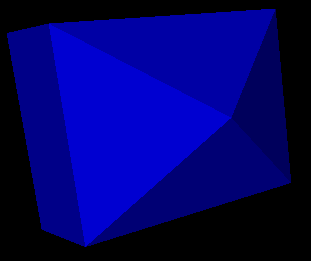
\includegraphics[scale=.2]{poly_1.png}
%% \end{minipage}
%% &
%% \begin{minipage}{.2\textwidth}
%% 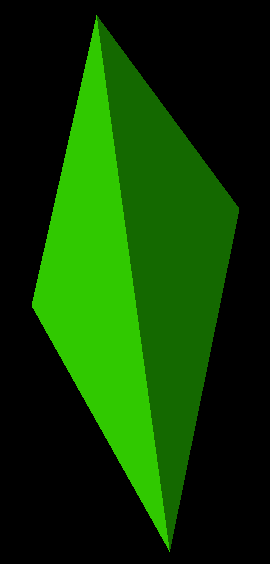
\includegraphics[scale=.2]{poly_2.png}
%% \end{minipage}
%% &
%% \begin{minipage}{.2\textwidth}
%% 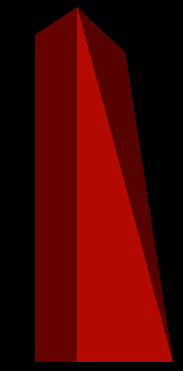
\includegraphics[scale=.2]{poly_3.png}
%% \end{minipage}
%% &
%% \begin{minipage}{.2\textwidth}
%% 
\includegraphics[scale=.2]{poly_4.png}
%% \end{minipage}
%% \\
%% \begin{minipage}{.2\textwidth}
%% 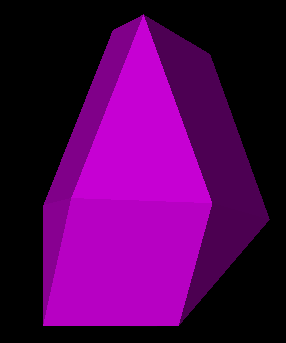
\includegraphics[scale=.2]{poly_5.png}
%% \end{minipage}
%% &
%% \begin{minipage}{.2\textwidth}
%% 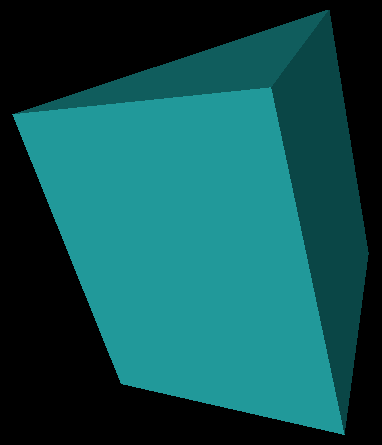
\includegraphics[scale=.2]{poly_6.png}
%% \end{minipage}
%% &
%% \begin{minipage}{.2\textwidth}
%% 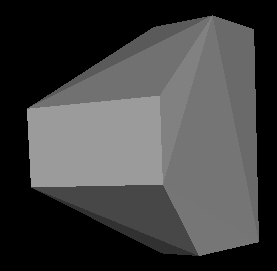
\includegraphics[scale=.2]{poly_7.png}
%% \end{minipage}
%% \end{tabular}
%% \end{center}
%% \caption{The polytopes that are to be packed.}
%% \label{fig:p}
%% \end{figure}

\begin{figure}
\begin{center}
\begin{tabular}{cc}
\begin{minipage}{.4\textwidth}
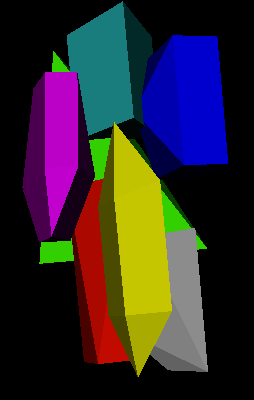
\includegraphics[scale=.5]{problem_7_1.png}
\end{minipage}
&
\begin{minipage}{.4\textwidth}
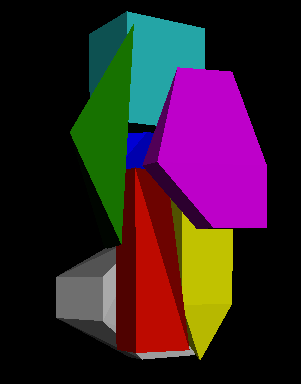
\includegraphics[scale=.5]{problem_7_2.png}
\end{minipage}
\end{tabular}
\end{center}
\caption{Two views of the packing placement for 7 polytopes as per~\cite{sto03} 
for a height of 23.}
\label{fig:p7}
\end{figure}

\section{Conclusion}

\bibliography{biblio}
\bibliographystyle{plain}
\end{document}
